\chapter{Statistical models}
Now that data is cleaned and prepared, a statistical analysis consisting of data segmentation and linear regression models can be made. The purpose of the analysis is to detect which attributes affects the performance of a specific house. 

\section{Linear regression}
Linear regression is a method to model the relationship between a dependent variable and one or more independent variables where the unknown model parameters are estimated from the data. \textcolor{red}{Mangler nok lidt her.} With the dependent variable $Y$ and the independent variables $x_1, \dots, x_n$, the linear regression model is formulated as 
\begin{equation}
    Y_i = \beta_0 + \beta_1 x_{i,1} + \beta_2 x_{i,2} + \cdots + \beta_p x_{i,p} + \varepsilon_i, \quad \varepsilon_i ~ \mathcal{N}(0,\sigma^2), \quad i = 1,\dots, n. \label{lm}
\end{equation}
The variables $\varepsilon_i$ are errors which are assumed to be white noise while also being i.i.d (independent and identically distributed). Equation \eqref{lm} shows a multiple linear regression model as it contains more than one explanatory variable. In this section both a simple linear model and a multiple linear model has been fitted to data given in table \ref{tab: modeldata}. 

\noindent As the best linear model $Y_i$ is desired, the total deviation from the data has to be as small as possible. The least squares method given as 
\begin{equation}
    \text{SSE} = \sum_{i=1}^n (Y_i - (\beta_0 + \beta_1 x_{i,1} + \beta_2 x_{i,2} + \cdots  \beta_p x_{i,p}))^2 = \sum_{i=1}^n (Y_i - \Hat{Y}_i)^2 
\end{equation} 
is chosen for estimating the model. The parameters $\beta_j$ are optimized to minimize the sum of squared errors of prediction (SSE).

\subsection{Model assumptions}
\noindent When SSE is minimized the model needs to be validated by checking whether the underlying model assumptions are fulfilled. 
\begin{enumerate} [label=\textbf{\arabic*}]
    \item Normality of residuals 
    \item Variance homogenity
    \item Variance should be independent of location
    \item Linear relationship between $x_j$ and $Y$
\end{enumerate}
If these assumptions are not met \textcolor{red}{\dots} \\

\noindent The fitting of the regression models is carried out by using the method stepwise regression \textcolor{red}{Bruger vi adjusted R-squared?} which updates the model in each step. In each step it is considered whether a variable is added or subtracted from the set of explanatory variables based on specific criteria. \\

\noindent Both a simple linear and a multiple linear regression model will be implemented in order to detect which attributes affect the performance of a specific house. This will be done by interpreting the estimates of the relation between the different explanatory attributes and \texttt{Consumption}. As mentioned, the p-value of the estimates of the explanatory variables will be the main focus when investigating which attributes influence the performance. 

\section{Simple linear regression model}
A simple linear regression model is fitted to each house with \texttt{Consumption} as a function of \texttt{Temperature}. Since it is expected that the temperature is the physical phenomenon with the greatest influence on the heat consumption, it is chosen as the independent variable. The models are performed by using the \texttt{lm()} function. The models will then be validated by examining whether the model assumptions in Chapter 4.1.1 are met. \\

\noindent 

\subsection{Results}
\begin{figure}
    \centering
    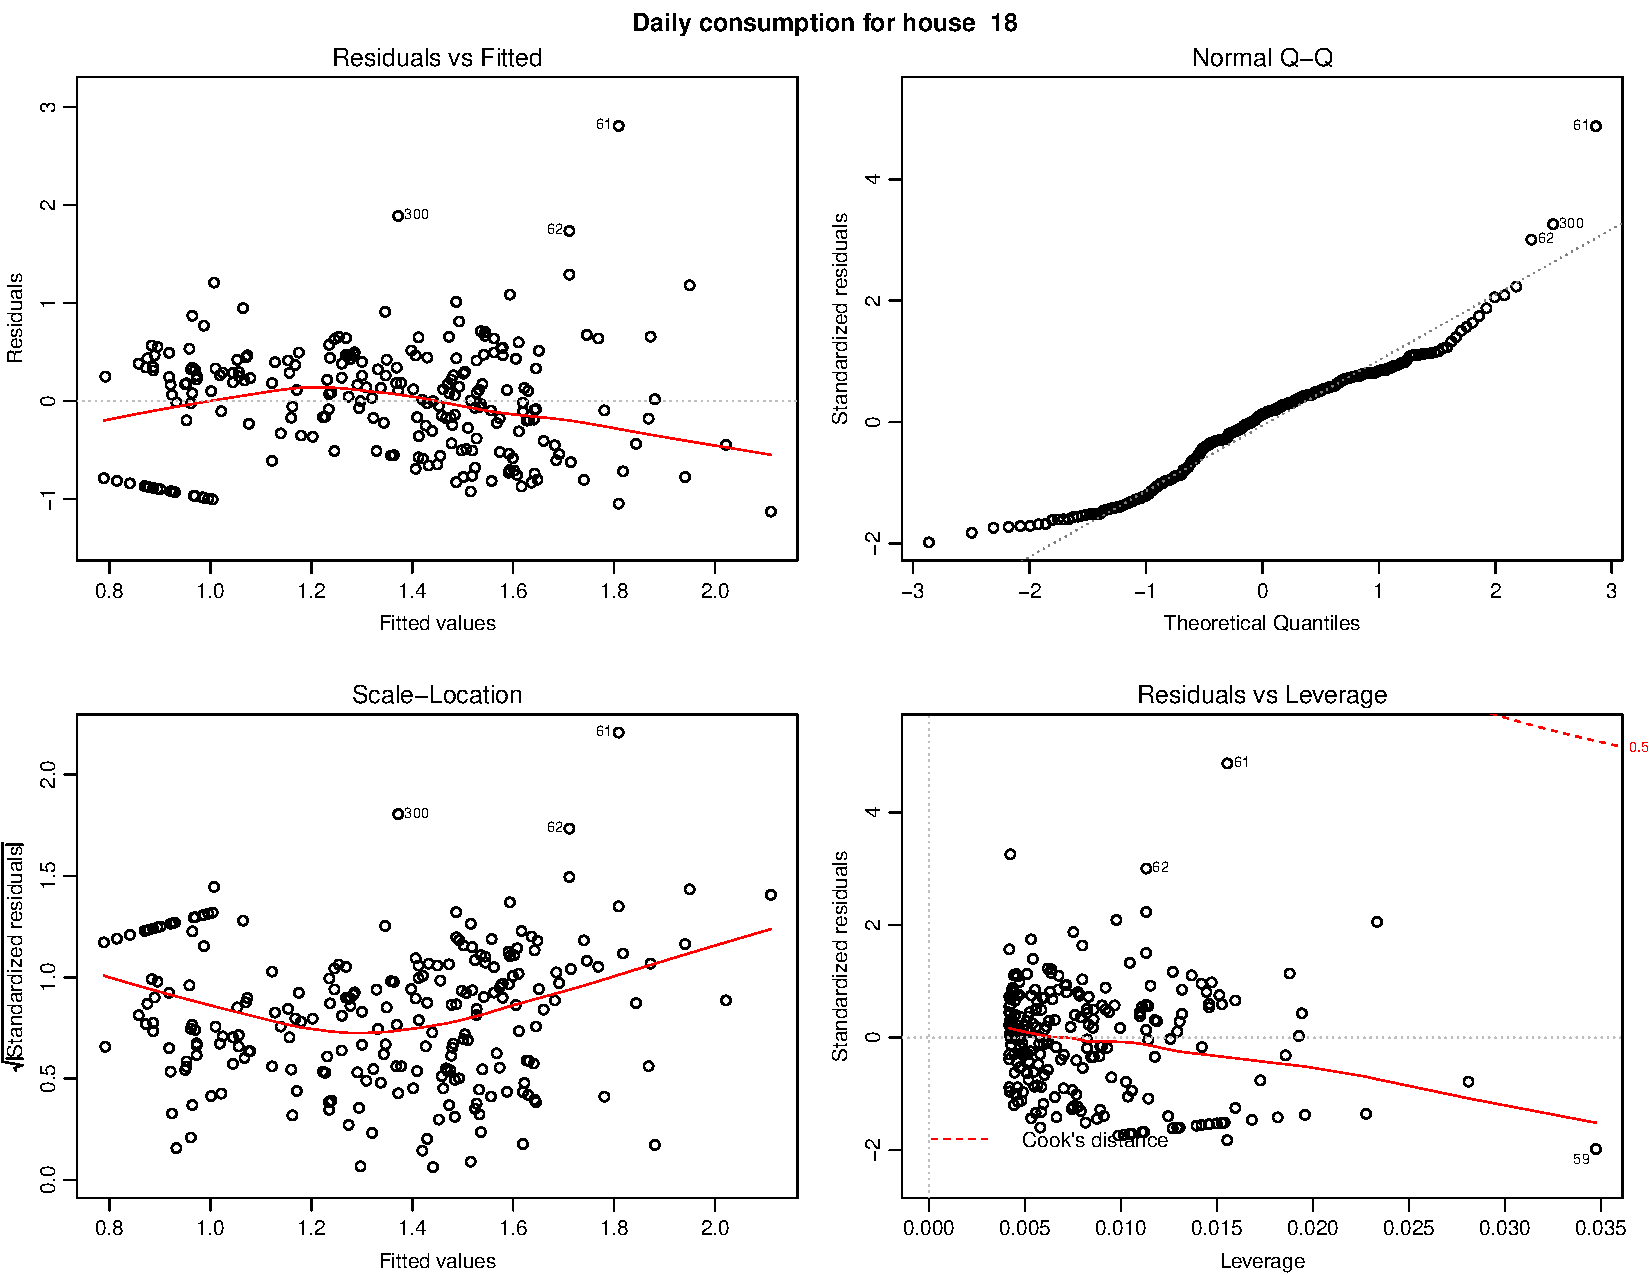
\includegraphics[width=.8\textwidth]{../../../figures/simple_lm18.pdf}
    \caption{}
    \label{fig: simple_lm_18}
\end{figure}

\section{Multiple linear regression model}

\textcolor{red}{Da alle attributter er gennemsnitlige for at få dagsværdier, giver condition ikke rigtig mening at have med i modellen. Derfor undlades den for nu.}

Vi medtager ikke interactions mellem holiday attributen og de andre attributter, da dette ikke er main focus. 

\subsection{Splines}
In the multiple regression model, splines will be used to model the wind direction. It does not make much sence to include the wind direction as it is in the model. It is not useful to know how significant the wind direction is, if it is not connected to the wind speed and if it is not known which directions are important. By modeling the wind direction with splines, each spline will represent a specific general direction.

Modellere wind direction
Lave en parameter om til flere vind retninger.
2. degree splines
Knots
Mellem retningerne
Giver mere mening for brugeren

\textcolor{red}{Vi vil gerne vægte vores vind i forskellige retninger i vores model, så derfor bruger vi splines til at modellere de forskellige retninger.} \\

\textcolor{red}{Tilføj billede af splines}

%\csvautotabular{lmMult_star.csv}

%\begin{table}
%    \centering
%    \begin{tabular}{cccccccccccc}%
%        \hline
%        & \bfseries I & \bfseries T & \bfseries N &\bfseries E & \bfseries S & \bfseries W & \bfseries SolaR & \bfseries T:N & \bfseries T:E & \bfseries T:S & \bfseries T:W \\
%        \hline
%        \csvreader[head to column names]{lmMult_star.csv}{}% use head of csv as column names
%        {\\\hline\I&\T&\N&\E&\S&\W&\SolaR&\T$:$N&\T$:$E&\T$:$S&\T$:$W}% specify your coloumns here
%    \end{tabular}
%    \caption{Table showing all players.}
%    \label{}
%\end{table}

%\begin{table}
%    \centering
%    \begin{tabular}{cccccccccccccc}
%        \hline
%        & \bfseries I & \bfseries T & \bfseries N &\bfseries E & \bfseries S & \bfseries W & \bfseries SolaR & \bfseries T:N & \bfseries T:E & \bfseries T:S & \bfseries T:W \\
%        \hline
%        1 & $\Plus \ast\ast\ast$	& $\Minus \ast \ast \ast$ & $\Plus$ & $\Plus$	& $\Plus$	& $\Plus \ast \ast$	& $\Minus$	& $\Plus$	& $\Minus$ & $\Plus$	& $\Minus \ast \ast$ \\
%        2 & $\Plus \ast \ast \ast$	& $\Minus \ast \ast \ast$ & $\Plus$ & $\Plus \ast \ast$	& $\Plus$	& $\Plus \ast \ast \ast$	& $\Minus \ast \ast \ast$	& $\Minus$	& $\Plus$ & $\Plus$	& $\Minus \ast \ast \ast$ \\
%        3 & $\Plus \ast \ast \ast$	& $\Minus \ast \ast \ast$ & $\Plus$ & $\Plus\ast\ast\ast$	& $\Plus$	& $\Plus \ast \ast\ast$	& $\Minus\ast\ast\ast$	& $\Minus$	& $\Minus$ & $\Plus\ast$	& $\Minus \ast$ \\
%        4 & \\
%        5 & \\
%        6 & \\
%        7 & \\
%        8 & \\
%        9 & \\
%        10 & \\
%        11 & \\
%        12 & \\
%        13 & \\
%        14 & \\
%        15 & \\
%        16 & \\
%        17 & \\
%        18 & \\
%        19 & \\
%        20 & \\
%        21 & \\
%        22 & \\
%        23 & \\
%        24 & \\
%        25 & \\
%        26 & \\
%        27 & \\
%        28 & \\
%        29 & \\
%        30 & \\
%        31 & \\
%        32 & \\
%        33 & \\
%        34 & \\
%        35 & \\
%        36 & \\
%        37 & \\
%        38 & \\
%        39 & \\
%        40 & \\
%        41 & \\
%        42 & \\
%        43 & \\
%        44 & \\
%        45 & \\
%        46 & \\
%        47 & \\
%        48 & \\
%        49 & \\
%        50 & \\
%        51 & \\
%        52 & \\
%        53 & \\
%        54 & \\
%        55 & \\
%        56 & \\
%        57 & \\
%        58 & \\
%        59 & \\
%        60 & \\
%        61 & \\
%        62 & \\
%        63 & \\
%        64 & \\
%        65 & \\
%        66 & \\
%        67 & \\
%        68 & \\
%        69 & \\
%        70 & \\
%        \hline
%    \end{tabular}
%    \caption{Table showing all games.}
%    \label{}
%\end{table}

\subsection{Results}

\section{Regression model for comparing houses}

\section{Comparison}